\documentclass[1p]{elsarticle_modified}
%\bibliographystyle{elsarticle-num}

%\usepackage[colorlinks]{hyperref}
%\usepackage{abbrmath_seonhwa} %\Abb, \Ascr, \Acal ,\Abf, \Afrak
\usepackage{amsfonts}
\usepackage{amssymb}
\usepackage{amsmath}
\usepackage{amsthm}
\usepackage{scalefnt}
\usepackage{amsbsy}
\usepackage{kotex}
\usepackage{caption}
\usepackage{subfig}
\usepackage{color}
\usepackage{graphicx}
\usepackage{xcolor} %% white, black, red, green, blue, cyan, magenta, yellow
\usepackage{float}
\usepackage{setspace}
\usepackage{hyperref}

\usepackage{tikz}
\usetikzlibrary{arrows}

\usepackage{multirow}
\usepackage{array} % fixed length table
\usepackage{hhline}

%%%%%%%%%%%%%%%%%%%%%
\makeatletter
\renewcommand*\env@matrix[1][\arraystretch]{%
	\edef\arraystretch{#1}%
	\hskip -\arraycolsep
	\let\@ifnextchar\new@ifnextchar
	\array{*\c@MaxMatrixCols c}}
\makeatother %https://tex.stackexchange.com/questions/14071/how-can-i-increase-the-line-spacing-in-a-matrix
%%%%%%%%%%%%%%%

\usepackage[normalem]{ulem}

\newcommand{\msout}[1]{\ifmmode\text{\sout{\ensuremath{#1}}}\else\sout{#1}\fi}
%SOURCE: \msout is \stkout macro in https://tex.stackexchange.com/questions/20609/strikeout-in-math-mode

\newcommand{\cancel}[1]{
	\ifmmode
	{\color{red}\msout{#1}}
	\else
	{\color{red}\sout{#1}}
	\fi
}

\newcommand{\add}[1]{
	{\color{blue}\uwave{#1}}
}

\newcommand{\replace}[2]{
	\ifmmode
	{\color{red}\msout{#1}}{\color{blue}\uwave{#2}}
	\else
	{\color{red}\sout{#1}}{\color{blue}\uwave{#2}}
	\fi
}

\newcommand{\Sol}{\mathcal{S}} %segment
\newcommand{\D}{D} %diagram
\newcommand{\A}{\mathcal{A}} %arc


%%%%%%%%%%%%%%%%%%%%%%%%%%%%%5 test

\def\sl{\operatorname{\textup{SL}}(2,\Cbb)}
\def\psl{\operatorname{\textup{PSL}}(2,\Cbb)}
\def\quan{\mkern 1mu \triangleright \mkern 1mu}

\theoremstyle{definition}
\newtheorem{thm}{Theorem}[section]
\newtheorem{prop}[thm]{Proposition}
\newtheorem{lem}[thm]{Lemma}
\newtheorem{ques}[thm]{Question}
\newtheorem{cor}[thm]{Corollary}
\newtheorem{defn}[thm]{Definition}
\newtheorem{exam}[thm]{Example}
\newtheorem{rmk}[thm]{Remark}
\newtheorem{alg}[thm]{Algorithm}

\newcommand{\I}{\sqrt{-1}}
\begin{document}

%\begin{frontmatter}
%
%\title{Boundary parabolic representations of knots up to 8 crossings}
%
%%% Group authors per affiliation:
%\author{Yunhi Cho} 
%\address{Department of Mathematics, University of Seoul, Seoul, Korea}
%\ead{yhcho@uos.ac.kr}
%
%
%\author{Seonhwa Kim} %\fnref{s_kim}}
%\address{Center for Geometry and Physics, Institute for Basic Science, Pohang, 37673, Korea}
%\ead{ryeona17@ibs.re.kr}
%
%\author{Hyuk Kim}
%\address{Department of Mathematical Sciences, Seoul National University, Seoul 08826, Korea}
%\ead{hyukkim@snu.ac.kr}
%
%\author{Seokbeom Yoon}
%\address{Department of Mathematical Sciences, Seoul National University, Seoul, 08826,  Korea}
%\ead{sbyoon15@snu.ac.kr}
%
%\begin{abstract}
%We find all boundary parabolic representation of knots up to 8 crossings.
%
%\end{abstract}
%\begin{keyword}
%    \MSC[2010] 57M25 
%\end{keyword}
%
%\end{frontmatter}

%\linenumbers
%\tableofcontents
%
\newcommand\colored[1]{\textcolor{white}{\rule[-0.35ex]{0.8em}{1.4ex}}\kern-0.8em\color{red} #1}%
%\newcommand\colored[1]{\textcolor{white}{ #1}\kern-2.17ex	\textcolor{white}{ #1}\kern-1.81ex	\textcolor{white}{ #1}\kern-2.15ex\color{red}#1	}

{\Large $\underline{11a_{169}~(K11a_{169})}$}

\setlength{\tabcolsep}{10pt}
\renewcommand{\arraystretch}{1.6}
\vspace{1cm}\begin{tabular}{m{100pt}>{\centering\arraybackslash}m{274pt}}
\multirow{5}{120pt}{
	\centering
	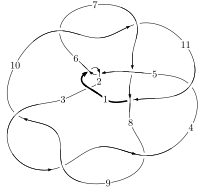
\includegraphics[width=112pt]{../../../GIT/diagram.site/Diagrams/png/418_11a_169.png}\\
\ \ \ A knot diagram\footnotemark}&
\allowdisplaybreaks
\textbf{Linearized knot diagam} \\
\cline{2-2}
 &
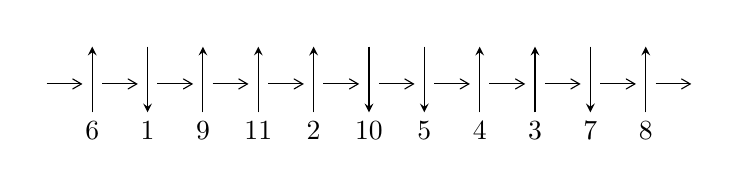
\begin{tikzpicture}[x=20pt, y=17pt]
	% nodes
	\node (C0) at (0, 0) {};
	\node (C1) at (1, 0) {};
	\node (C1U) at (1, +1) {};
	\node (C1D) at (1, -1) {6};

	\node (C2) at (2, 0) {};
	\node (C2U) at (2, +1) {};
	\node (C2D) at (2, -1) {1};

	\node (C3) at (3, 0) {};
	\node (C3U) at (3, +1) {};
	\node (C3D) at (3, -1) {9};

	\node (C4) at (4, 0) {};
	\node (C4U) at (4, +1) {};
	\node (C4D) at (4, -1) {11};

	\node (C5) at (5, 0) {};
	\node (C5U) at (5, +1) {};
	\node (C5D) at (5, -1) {2};

	\node (C6) at (6, 0) {};
	\node (C6U) at (6, +1) {};
	\node (C6D) at (6, -1) {10};

	\node (C7) at (7, 0) {};
	\node (C7U) at (7, +1) {};
	\node (C7D) at (7, -1) {5};

	\node (C8) at (8, 0) {};
	\node (C8U) at (8, +1) {};
	\node (C8D) at (8, -1) {4};

	\node (C9) at (9, 0) {};
	\node (C9U) at (9, +1) {};
	\node (C9D) at (9, -1) {3};

	\node (C10) at (10, 0) {};
	\node (C10U) at (10, +1) {};
	\node (C10D) at (10, -1) {7};

	\node (C11) at (11, 0) {};
	\node (C11U) at (11, +1) {};
	\node (C11D) at (11, -1) {8};
	\node (C12) at (12, 0) {};

	% arrows
	\draw[->,>={angle 60}]
	(C0) edge (C1) (C1) edge (C2) (C2) edge (C3) (C3) edge (C4) (C4) edge (C5) (C5) edge (C6) (C6) edge (C7) (C7) edge (C8) (C8) edge (C9) (C9) edge (C10) (C10) edge (C11) (C11) edge (C12) ;	\draw[->,>=stealth]
	(C1D) edge (C1U) (C2U) edge (C2D) (C3D) edge (C3U) (C4D) edge (C4U) (C5D) edge (C5U) (C6U) edge (C6D) (C7U) edge (C7D) (C8D) edge (C8U) (C9D) edge (C9U) (C10U) edge (C10D) (C11D) edge (C11U) ;
	\end{tikzpicture} \\
\hhline{~~} \\& 
\textbf{Solving Sequence} \\ \cline{2-2} 
 &
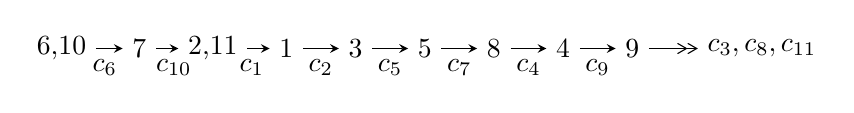
\begin{tikzpicture}[x=25pt, y=7pt]
	% node
	\node (A0) at (-1/8, 0) {6,10};
	\node (A1) at (1, 0) {7};
	\node (A2) at (33/16, 0) {2,11};
	\node (A3) at (25/8, 0) {1};
	\node (A4) at (33/8, 0) {3};
	\node (A5) at (41/8, 0) {5};
	\node (A6) at (49/8, 0) {8};
	\node (A7) at (57/8, 0) {4};
	\node (A8) at (65/8, 0) {9};
	\node (C1) at (1/2, -1) {$c_{6}$};
	\node (C2) at (3/2, -1) {$c_{10}$};
	\node (C3) at (21/8, -1) {$c_{1}$};
	\node (C4) at (29/8, -1) {$c_{2}$};
	\node (C5) at (37/8, -1) {$c_{5}$};
	\node (C6) at (45/8, -1) {$c_{7}$};
	\node (C7) at (53/8, -1) {$c_{4}$};
	\node (C8) at (61/8, -1) {$c_{9}$};
	\node (A9) at (10, 0) {$c_{3},c_{8},c_{11}$};

	% edge
	\draw[->,>=stealth]	
	(A0) edge (A1) (A1) edge (A2) (A2) edge (A3) (A3) edge (A4) (A4) edge (A5) (A5) edge (A6) (A6) edge (A7) (A7) edge (A8) ;
	\draw[->>,>={angle 60}]	
	(A8) edge (A9);
\end{tikzpicture} \\ 

\end{tabular} \\

\footnotetext{
The image of knot diagram is generated by the software ``\textbf{Draw programme}" developed by Andrew Bartholomew(\url{http://www.layer8.co.uk/maths/draw/index.htm\#Running-draw}), where we modified some parts for our purpose(\url{https://github.com/CATsTAILs/LinksPainter}).
}\phantom \\ \newline 
\centering \textbf{Ideals for irreducible components\footnotemark of $X_{\text{par}}$} 
 
\begin{align*}
I^u_{1}&=\langle 
-4.96166\times10^{185} u^{73}+1.25507\times10^{186} u^{72}+\cdots+1.38036\times10^{187} b-2.21942\times10^{187},\\
\phantom{I^u_{1}}&\phantom{= \langle  }5.60840\times10^{187} u^{73}-1.03180\times10^{188} u^{72}+\cdots+5.10733\times10^{188} a+2.81879\times10^{189},\;u^{74}- u^{73}+\cdots+36 u+37\rangle \\
I^u_{2}&=\langle 
4 u^{13}+7 u^{12}-21 u^{11}-33 u^{10}+49 u^9+71 u^8-56 u^7-90 u^6+36 u^5+66 u^4-4 u^3-26 u^2+b-3 u+4,\\
\phantom{I^u_{2}}&\phantom{= \langle  }6 u^{13}+10 u^{12}+\cdots+a+10,\\
\phantom{I^u_{2}}&\phantom{= \langle  }u^{14}+2 u^{13}-5 u^{12}-10 u^{11}+11 u^{10}+23 u^9-11 u^8-31 u^7+4 u^6+25 u^5+4 u^4-11 u^3-4 u^2+2 u+1\rangle \\
\\
\end{align*}
\raggedright * 2 irreducible components of $\dim_{\mathbb{C}}=0$, with total 88 representations.\\
\footnotetext{All coefficients of polynomials are rational numbers. But the coefficients are sometimes approximated in decimal forms when there is not enough margin.}
\newpage
\renewcommand{\arraystretch}{1}
\centering \section*{I. $I^u_{1}= \langle -4.96\times10^{185} u^{73}+1.26\times10^{186} u^{72}+\cdots+1.38\times10^{187} b-2.22\times10^{187},\;5.61\times10^{187} u^{73}-1.03\times10^{188} u^{72}+\cdots+5.11\times10^{188} a+2.82\times10^{189},\;u^{74}- u^{73}+\cdots+36 u+37 \rangle$}
\flushleft \textbf{(i) Arc colorings}\\
\begin{tabular}{m{7pt} m{180pt} m{7pt} m{180pt} }
\flushright $a_{6}=$&$\begin{pmatrix}1\\0\end{pmatrix}$ \\
\flushright $a_{10}=$&$\begin{pmatrix}0\\u\end{pmatrix}$ \\
\flushright $a_{7}=$&$\begin{pmatrix}1\\u^2\end{pmatrix}$ \\
\flushright $a_{2}=$&$\begin{pmatrix}-0.109811 u^{73}+0.202024 u^{72}+\cdots-3.01507 u-5.51912\\0.0359447 u^{73}-0.0909234 u^{72}+\cdots-0.656044 u+1.60786\end{pmatrix}$ \\
\flushright $a_{11}=$&$\begin{pmatrix}- u\\- u^3+u\end{pmatrix}$ \\
\flushright $a_{1}=$&$\begin{pmatrix}-0.145756 u^{73}+0.292948 u^{72}+\cdots-2.35903 u-7.12697\\0.0359447 u^{73}-0.0909234 u^{72}+\cdots-0.656044 u+1.60786\end{pmatrix}$ \\
\flushright $a_{3}=$&$\begin{pmatrix}0.107346 u^{73}-0.195541 u^{72}+\cdots-2.58294 u+3.70574\\-0.318159 u^{73}+0.662604 u^{72}+\cdots-2.83612 u-10.4308\end{pmatrix}$ \\
\flushright $a_{5}=$&$\begin{pmatrix}-0.187310 u^{73}+0.380215 u^{72}+\cdots-4.71712 u-5.98298\\0.0710115 u^{73}-0.143579 u^{72}+\cdots-2.35575 u+2.65479\end{pmatrix}$ \\
\flushright $a_{8}=$&$\begin{pmatrix}-0.168216 u^{73}+0.379034 u^{72}+\cdots+3.07123 u-4.69178\\-0.0865870 u^{73}+0.159014 u^{72}+\cdots+1.12473 u-4.45130\end{pmatrix}$ \\
\flushright $a_{4}=$&$\begin{pmatrix}-0.284387 u^{73}+0.587033 u^{72}+\cdots-4.79088 u-9.08039\\0.0463239 u^{73}-0.104793 u^{72}+\cdots-2.64081 u+1.69178\end{pmatrix}$ \\
\flushright $a_{9}=$&$\begin{pmatrix}0.0959357 u^{73}-0.265994 u^{72}+\cdots+1.34312 u+0.825831\\-0.160387 u^{73}+0.335587 u^{72}+\cdots+1.38132 u-5.82341\end{pmatrix}$\\ \flushright $a_{9}=$&$\begin{pmatrix}0.0959357 u^{73}-0.265994 u^{72}+\cdots+1.34312 u+0.825831\\-0.160387 u^{73}+0.335587 u^{72}+\cdots+1.38132 u-5.82341\end{pmatrix}$\\&\end{tabular}
\flushleft \textbf{(ii) Obstruction class $= -1$}\\~\\
\flushleft \textbf{(iii) Cusp Shapes $= -0.581332 u^{73}+1.19718 u^{72}+\cdots+15.2381 u-18.9875$}\\~\\
\newpage\renewcommand{\arraystretch}{1}
\flushleft \textbf{(iv) u-Polynomials at the component}\newline \\
\begin{tabular}{m{50pt}|m{274pt}}
Crossings & \hspace{64pt}u-Polynomials at each crossing \\
\hline $$\begin{aligned}c_{1},c_{5}\end{aligned}$$&$\begin{aligned}
&u^{74}+18 u^{72}+\cdots+5 u+1
\end{aligned}$\\
\hline $$\begin{aligned}c_{2}\end{aligned}$$&$\begin{aligned}
&u^{74}+36 u^{73}+\cdots-17 u+1
\end{aligned}$\\
\hline $$\begin{aligned}c_{3},c_{8},c_{9}\end{aligned}$$&$\begin{aligned}
&u^{74}- u^{73}+\cdots+22 u+1
\end{aligned}$\\
\hline $$\begin{aligned}c_{4}\end{aligned}$$&$\begin{aligned}
&u^{74}-3 u^{73}+\cdots-176 u+1003
\end{aligned}$\\
\hline $$\begin{aligned}c_{6},c_{10}\end{aligned}$$&$\begin{aligned}
&u^{74}- u^{73}+\cdots+36 u+37
\end{aligned}$\\
\hline $$\begin{aligned}c_{7}\end{aligned}$$&$\begin{aligned}
&u^{74}-5 u^{73}+\cdots-20 u+1
\end{aligned}$\\
\hline $$\begin{aligned}c_{11}\end{aligned}$$&$\begin{aligned}
&u^{74}-5 u^{73}+\cdots+300 u+125
\end{aligned}$\\
\hline
\end{tabular}\\~\\
\newpage\renewcommand{\arraystretch}{1}
\flushleft \textbf{(v) Riley Polynomials at the component}\newline \\
\begin{tabular}{m{50pt}|m{274pt}}
Crossings & \hspace{64pt}Riley Polynomials at each crossing \\
\hline $$\begin{aligned}c_{1},c_{5}\end{aligned}$$&$\begin{aligned}
&y^{74}+36 y^{73}+\cdots-17 y+1
\end{aligned}$\\
\hline $$\begin{aligned}c_{2}\end{aligned}$$&$\begin{aligned}
&y^{74}+12 y^{73}+\cdots-77 y+1
\end{aligned}$\\
\hline $$\begin{aligned}c_{3},c_{8},c_{9}\end{aligned}$$&$\begin{aligned}
&y^{74}+77 y^{73}+\cdots-58 y+1
\end{aligned}$\\
\hline $$\begin{aligned}c_{4}\end{aligned}$$&$\begin{aligned}
&y^{74}+29 y^{73}+\cdots+34287672 y+1006009
\end{aligned}$\\
\hline $$\begin{aligned}c_{6},c_{10}\end{aligned}$$&$\begin{aligned}
&y^{74}-57 y^{73}+\cdots-4034 y+1369
\end{aligned}$\\
\hline $$\begin{aligned}c_{7}\end{aligned}$$&$\begin{aligned}
&y^{74}-9 y^{73}+\cdots+14 y+1
\end{aligned}$\\
\hline $$\begin{aligned}c_{11}\end{aligned}$$&$\begin{aligned}
&y^{74}+15 y^{73}+\cdots+308750 y+15625
\end{aligned}$\\
\hline
\end{tabular}\\~\\
\newpage\flushleft \textbf{(vi) Complex Volumes and Cusp Shapes}
$$\begin{array}{c|c|c}  
\text{Solutions to }I^u_{1}& \I (\text{vol} + \sqrt{-1}CS) & \text{Cusp shape}\\
 \hline 
\begin{aligned}
u &= -0.041401 + 1.026520 I \\
a &= \phantom{-}0.661998 - 0.676360 I \\
b &= -0.590855 - 0.983471 I\end{aligned}
 & \phantom{-}1.11109 + 6.26090 I & \phantom{-0.000000 } 0 \\ \hline\begin{aligned}
u &= -0.041401 - 1.026520 I \\
a &= \phantom{-}0.661998 + 0.676360 I \\
b &= -0.590855 + 0.983471 I\end{aligned}
 & \phantom{-}1.11109 - 6.26090 I & \phantom{-0.000000 } 0 \\ \hline\begin{aligned}
u &= -0.986532 + 0.392792 I \\
a &= \phantom{-}0.390575 - 0.412307 I \\
b &= -0.201955 - 0.077354 I\end{aligned}
 & -1.70214 + 1.37634 I & \phantom{-0.000000 } 0 \\ \hline\begin{aligned}
u &= -0.986532 - 0.392792 I \\
a &= \phantom{-}0.390575 + 0.412307 I \\
b &= -0.201955 + 0.077354 I\end{aligned}
 & -1.70214 - 1.37634 I & \phantom{-0.000000 } 0 \\ \hline\begin{aligned}
u &= -1.064540 + 0.083077 I \\
a &= -0.038681 - 0.719869 I \\
b &= -1.066260 - 0.903808 I\end{aligned}
 & -3.93189 + 3.73813 I & \phantom{-0.000000 } 0 \\ \hline\begin{aligned}
u &= -1.064540 - 0.083077 I \\
a &= -0.038681 + 0.719869 I \\
b &= -1.066260 + 0.903808 I\end{aligned}
 & -3.93189 - 3.73813 I & \phantom{-0.000000 } 0 \\ \hline\begin{aligned}
u &= -0.054647 + 1.089920 I \\
a &= -0.798538 + 0.520307 I \\
b &= \phantom{-}0.662690 + 0.358460 I\end{aligned}
 & -3.49876 - 4.45579 I & \phantom{-0.000000 } 0 \\ \hline\begin{aligned}
u &= -0.054647 - 1.089920 I \\
a &= -0.798538 - 0.520307 I \\
b &= \phantom{-}0.662690 - 0.358460 I\end{aligned}
 & -3.49876 + 4.45579 I & \phantom{-0.000000 } 0 \\ \hline\begin{aligned}
u &= \phantom{-}1.008160 + 0.419741 I \\
a &= -1.13208 - 2.49760 I \\
b &= \phantom{-}0.086823 - 0.942517 I\end{aligned}
 & -5.90718 - 3.61297 I & \phantom{-0.000000 } 0 \\ \hline\begin{aligned}
u &= \phantom{-}1.008160 - 0.419741 I \\
a &= -1.13208 + 2.49760 I \\
b &= \phantom{-}0.086823 + 0.942517 I\end{aligned}
 & -5.90718 + 3.61297 I & \phantom{-0.000000 } 0\\
 \hline 
 \end{array}$$\newpage$$\begin{array}{c|c|c}  
\text{Solutions to }I^u_{1}& \I (\text{vol} + \sqrt{-1}CS) & \text{Cusp shape}\\
 \hline 
\begin{aligned}
u &= \phantom{-}0.164060 + 0.892569 I \\
a &= \phantom{-}0.610647 + 0.324648 I \\
b &= -0.635278 + 0.581899 I\end{aligned}
 & \phantom{-}2.28203 + 1.45434 I & \phantom{-}7.07609 - 2.82697 I \\ \hline\begin{aligned}
u &= \phantom{-}0.164060 - 0.892569 I \\
a &= \phantom{-}0.610647 - 0.324648 I \\
b &= -0.635278 - 0.581899 I\end{aligned}
 & \phantom{-}2.28203 - 1.45434 I & \phantom{-}7.07609 + 2.82697 I \\ \hline\begin{aligned}
u &= -1.020520 + 0.447604 I \\
a &= \phantom{-}0.90579 - 1.99644 I \\
b &= -0.56045 - 1.35749 I\end{aligned}
 & -7.03134 + 7.38518 I & \phantom{-0.000000 } 0 \\ \hline\begin{aligned}
u &= -1.020520 - 0.447604 I \\
a &= \phantom{-}0.90579 + 1.99644 I \\
b &= -0.56045 + 1.35749 I\end{aligned}
 & -7.03134 - 7.38518 I & \phantom{-0.000000 } 0 \\ \hline\begin{aligned}
u &= -0.706637 + 0.528963 I \\
a &= \phantom{-}0.715385 + 0.015552 I \\
b &= -0.111730 + 0.682639 I\end{aligned}
 & -1.94267 + 1.36984 I & -1.20938 - 5.61656 I \\ \hline\begin{aligned}
u &= -0.706637 - 0.528963 I \\
a &= \phantom{-}0.715385 - 0.015552 I \\
b &= -0.111730 - 0.682639 I\end{aligned}
 & -1.94267 - 1.36984 I & -1.20938 + 5.61656 I \\ \hline\begin{aligned}
u &= -1.118000 + 0.053349 I \\
a &= -1.16980 + 2.42638 I \\
b &= \phantom{-}0.427319 + 1.057150 I\end{aligned}
 & -3.93201 + 1.54935 I & \phantom{-0.000000 } 0 \\ \hline\begin{aligned}
u &= -1.118000 - 0.053349 I \\
a &= -1.16980 - 2.42638 I \\
b &= \phantom{-}0.427319 - 1.057150 I\end{aligned}
 & -3.93201 - 1.54935 I & \phantom{-0.000000 } 0 \\ \hline\begin{aligned}
u &= \phantom{-}1.094100 + 0.269644 I \\
a &= -0.50567 - 2.00641 I \\
b &= \phantom{-}0.561390 - 1.183450 I\end{aligned}
 & -1.87663 - 4.80358 I & \phantom{-0.000000 } 0 \\ \hline\begin{aligned}
u &= \phantom{-}1.094100 - 0.269644 I \\
a &= -0.50567 + 2.00641 I \\
b &= \phantom{-}0.561390 + 1.183450 I\end{aligned}
 & -1.87663 + 4.80358 I & \phantom{-0.000000 } 0\\
 \hline 
 \end{array}$$\newpage$$\begin{array}{c|c|c}  
\text{Solutions to }I^u_{1}& \I (\text{vol} + \sqrt{-1}CS) & \text{Cusp shape}\\
 \hline 
\begin{aligned}
u &= -0.716202 + 0.466840 I \\
a &= -0.082574 - 0.910018 I \\
b &= -0.902862 - 0.142948 I\end{aligned}
 & -2.54067 + 2.00646 I & \phantom{-}4.56819 - 2.62899 I \\ \hline\begin{aligned}
u &= -0.716202 - 0.466840 I \\
a &= -0.082574 + 0.910018 I \\
b &= -0.902862 + 0.142948 I\end{aligned}
 & -2.54067 - 2.00646 I & \phantom{-}4.56819 + 2.62899 I \\ \hline\begin{aligned}
u &= -0.453990 + 0.701764 I \\
a &= -0.330021 + 0.379368 I \\
b &= -0.539990 + 1.146080 I\end{aligned}
 & -5.37822 - 3.01874 I & -1.04024 + 2.49965 I \\ \hline\begin{aligned}
u &= -0.453990 - 0.701764 I \\
a &= -0.330021 - 0.379368 I \\
b &= -0.539990 - 1.146080 I\end{aligned}
 & -5.37822 + 3.01874 I & -1.04024 - 2.49965 I \\ \hline\begin{aligned}
u &= \phantom{-}1.150740 + 0.216584 I \\
a &= -0.08189 - 2.43504 I \\
b &= -0.150667 - 1.122100 I\end{aligned}
 & -6.13754 - 3.74072 I & \phantom{-0.000000 } 0 \\ \hline\begin{aligned}
u &= \phantom{-}1.150740 - 0.216584 I \\
a &= -0.08189 + 2.43504 I \\
b &= -0.150667 + 1.122100 I\end{aligned}
 & -6.13754 + 3.74072 I & \phantom{-0.000000 } 0 \\ \hline\begin{aligned}
u &= -1.109710 + 0.388330 I \\
a &= \phantom{-}0.698876 - 0.299047 I \\
b &= \phantom{-}0.340968 - 0.383433 I\end{aligned}
 & -1.55302 + 1.40337 I & \phantom{-0.000000 } 0 \\ \hline\begin{aligned}
u &= -1.109710 - 0.388330 I \\
a &= \phantom{-}0.698876 + 0.299047 I \\
b &= \phantom{-}0.340968 + 0.383433 I\end{aligned}
 & -1.55302 - 1.40337 I & \phantom{-0.000000 } 0 \\ \hline\begin{aligned}
u &= \phantom{-}1.191070 + 0.010518 I \\
a &= -0.022094 + 0.440729 I \\
b &= -0.772060 - 0.401516 I\end{aligned}
 & -7.86764 - 1.80141 I & \phantom{-0.000000 } 0 \\ \hline\begin{aligned}
u &= \phantom{-}1.191070 - 0.010518 I \\
a &= -0.022094 - 0.440729 I \\
b &= -0.772060 + 0.401516 I\end{aligned}
 & -7.86764 + 1.80141 I & \phantom{-0.000000 } 0\\
 \hline 
 \end{array}$$\newpage$$\begin{array}{c|c|c}  
\text{Solutions to }I^u_{1}& \I (\text{vol} + \sqrt{-1}CS) & \text{Cusp shape}\\
 \hline 
\begin{aligned}
u &= \phantom{-}1.189310 + 0.229765 I \\
a &= \phantom{-}1.31840 + 1.49765 I \\
b &= -0.583679 + 1.119390 I\end{aligned}
 & -10.02310 - 6.93733 I & \phantom{-0.000000 } 0 \\ \hline\begin{aligned}
u &= \phantom{-}1.189310 - 0.229765 I \\
a &= \phantom{-}1.31840 - 1.49765 I \\
b &= -0.583679 - 1.119390 I\end{aligned}
 & -10.02310 + 6.93733 I & \phantom{-0.000000 } 0 \\ \hline\begin{aligned}
u &= \phantom{-}0.730409 + 0.234263 I \\
a &= \phantom{-}0.002848 - 0.948008 I \\
b &= \phantom{-}0.823183 - 0.768347 I\end{aligned}
 & \phantom{-}0.90646 - 3.01225 I & \phantom{-}11.02233 + 8.12268 I \\ \hline\begin{aligned}
u &= \phantom{-}0.730409 - 0.234263 I \\
a &= \phantom{-}0.002848 + 0.948008 I \\
b &= \phantom{-}0.823183 + 0.768347 I\end{aligned}
 & \phantom{-}0.90646 + 3.01225 I & \phantom{-}11.02233 - 8.12268 I \\ \hline\begin{aligned}
u &= \phantom{-}0.645449 + 1.130360 I \\
a &= -0.399107 + 0.201377 I \\
b &= \phantom{-}0.330428 + 1.061930 I\end{aligned}
 & -7.17177 - 2.00704 I & \phantom{-0.000000 } 0 \\ \hline\begin{aligned}
u &= \phantom{-}0.645449 - 1.130360 I \\
a &= -0.399107 - 0.201377 I \\
b &= \phantom{-}0.330428 - 1.061930 I\end{aligned}
 & -7.17177 + 2.00704 I & \phantom{-0.000000 } 0 \\ \hline\begin{aligned}
u &= -0.644097 + 0.246664 I \\
a &= -1.22405 + 1.11061 I \\
b &= -0.704733 + 0.577546 I\end{aligned}
 & -2.89873 - 2.58975 I & -0.111793 + 1.162954 I \\ \hline\begin{aligned}
u &= -0.644097 - 0.246664 I \\
a &= -1.22405 - 1.11061 I \\
b &= -0.704733 - 0.577546 I\end{aligned}
 & -2.89873 + 2.58975 I & -0.111793 - 1.162954 I \\ \hline\begin{aligned}
u &= \phantom{-}1.229030 + 0.471094 I \\
a &= -0.391923 + 0.075906 I \\
b &= -0.820281 - 0.357667 I\end{aligned}
 & -1.05855 - 6.36832 I & \phantom{-0.000000 } 0 \\ \hline\begin{aligned}
u &= \phantom{-}1.229030 - 0.471094 I \\
a &= -0.391923 - 0.075906 I \\
b &= -0.820281 + 0.357667 I\end{aligned}
 & -1.05855 + 6.36832 I & \phantom{-0.000000 } 0\\
 \hline 
 \end{array}$$\newpage$$\begin{array}{c|c|c}  
\text{Solutions to }I^u_{1}& \I (\text{vol} + \sqrt{-1}CS) & \text{Cusp shape}\\
 \hline 
\begin{aligned}
u &= -1.315060 + 0.070834 I \\
a &= \phantom{-}0.10565 + 1.58707 I \\
b &= -0.461958 + 1.011830 I\end{aligned}
 & -3.68119 - 1.72060 I & \phantom{-0.000000 } 0 \\ \hline\begin{aligned}
u &= -1.315060 - 0.070834 I \\
a &= \phantom{-}0.10565 - 1.58707 I \\
b &= -0.461958 - 1.011830 I\end{aligned}
 & -3.68119 + 1.72060 I & \phantom{-0.000000 } 0 \\ \hline\begin{aligned}
u &= -1.353880 + 0.256891 I \\
a &= -0.30501 + 2.26816 I \\
b &= \phantom{-}0.478617 + 1.068020 I\end{aligned}
 & -3.56136 + 5.27681 I & \phantom{-0.000000 } 0 \\ \hline\begin{aligned}
u &= -1.353880 - 0.256891 I \\
a &= -0.30501 - 2.26816 I \\
b &= \phantom{-}0.478617 - 1.068020 I\end{aligned}
 & -3.56136 - 5.27681 I & \phantom{-0.000000 } 0 \\ \hline\begin{aligned}
u &= \phantom{-}0.563652 + 0.233266 I \\
a &= \phantom{-}0.719862 - 0.170364 I \\
b &= \phantom{-}0.648787 + 0.161529 I\end{aligned}
 & \phantom{-}1.084040 + 0.054792 I & \phantom{-}10.18991 + 0.13008 I \\ \hline\begin{aligned}
u &= \phantom{-}0.563652 - 0.233266 I \\
a &= \phantom{-}0.719862 + 0.170364 I \\
b &= \phantom{-}0.648787 - 0.161529 I\end{aligned}
 & \phantom{-}1.084040 - 0.054792 I & \phantom{-}10.18991 - 0.13008 I \\ \hline\begin{aligned}
u &= -1.40158 + 0.28073 I \\
a &= \phantom{-}0.07621 - 1.71088 I \\
b &= \phantom{-}0.15964 - 1.41781 I\end{aligned}
 & -13.8677 + 6.0588 I & \phantom{-0.000000 } 0 \\ \hline\begin{aligned}
u &= -1.40158 - 0.28073 I \\
a &= \phantom{-}0.07621 + 1.71088 I \\
b &= \phantom{-}0.15964 + 1.41781 I\end{aligned}
 & -13.8677 - 6.0588 I & \phantom{-0.000000 } 0 \\ \hline\begin{aligned}
u &= -0.179516 + 0.523495 I \\
a &= -0.414147 - 0.312461 I \\
b &= \phantom{-}0.614780 + 0.802645 I\end{aligned}
 & \phantom{-}1.20853 + 2.22979 I & \phantom{-}5.58274 - 4.23366 I \\ \hline\begin{aligned}
u &= -0.179516 - 0.523495 I \\
a &= -0.414147 + 0.312461 I \\
b &= \phantom{-}0.614780 - 0.802645 I\end{aligned}
 & \phantom{-}1.20853 - 2.22979 I & \phantom{-}5.58274 + 4.23366 I\\
 \hline 
 \end{array}$$\newpage$$\begin{array}{c|c|c}  
\text{Solutions to }I^u_{1}& \I (\text{vol} + \sqrt{-1}CS) & \text{Cusp shape}\\
 \hline 
\begin{aligned}
u &= \phantom{-}0.03616 + 1.44649 I \\
a &= -0.485282 - 0.593135 I \\
b &= \phantom{-}0.540574 - 1.099130 I\end{aligned}
 & -5.65481 - 9.14282 I & \phantom{-0.000000 } 0 \\ \hline\begin{aligned}
u &= \phantom{-}0.03616 - 1.44649 I \\
a &= -0.485282 + 0.593135 I \\
b &= \phantom{-}0.540574 + 1.099130 I\end{aligned}
 & -5.65481 + 9.14282 I & \phantom{-0.000000 } 0 \\ \hline\begin{aligned}
u &= -1.29046 + 0.66405 I \\
a &= \phantom{-}0.98402 - 1.42129 I \\
b &= -0.450482 - 1.038080 I\end{aligned}
 & -3.68654 + 4.65688 I & \phantom{-0.000000 } 0 \\ \hline\begin{aligned}
u &= -1.29046 - 0.66405 I \\
a &= \phantom{-}0.98402 + 1.42129 I \\
b &= -0.450482 + 1.038080 I\end{aligned}
 & -3.68654 - 4.65688 I & \phantom{-0.000000 } 0 \\ \hline\begin{aligned}
u &= -1.35471 + 0.52687 I \\
a &= \phantom{-}0.231505 + 0.110886 I \\
b &= \phantom{-}1.018660 - 0.327910 I\end{aligned}
 & -7.66023 + 10.17330 I & \phantom{-0.000000 } 0 \\ \hline\begin{aligned}
u &= -1.35471 - 0.52687 I \\
a &= \phantom{-}0.231505 - 0.110886 I \\
b &= \phantom{-}1.018660 + 0.327910 I\end{aligned}
 & -7.66023 - 10.17330 I & \phantom{-0.000000 } 0 \\ \hline\begin{aligned}
u &= \phantom{-}1.37570 + 0.47899 I \\
a &= \phantom{-}0.73388 + 1.86660 I \\
b &= -0.588470 + 1.135700 I\end{aligned}
 & -3.38565 - 11.61060 I & \phantom{-0.000000 } 0 \\ \hline\begin{aligned}
u &= \phantom{-}1.37570 - 0.47899 I \\
a &= \phantom{-}0.73388 - 1.86660 I \\
b &= -0.588470 - 1.135700 I\end{aligned}
 & -3.38565 + 11.61060 I & \phantom{-0.000000 } 0 \\ \hline\begin{aligned}
u &= \phantom{-}1.36071 + 0.58544 I \\
a &= -0.320853 - 0.015899 I \\
b &= \phantom{-}0.748042 + 0.449545 I\end{aligned}
 & -7.59610 - 0.90779 I & \phantom{-0.000000 } 0 \\ \hline\begin{aligned}
u &= \phantom{-}1.36071 - 0.58544 I \\
a &= -0.320853 + 0.015899 I \\
b &= \phantom{-}0.748042 - 0.449545 I\end{aligned}
 & -7.59610 + 0.90779 I & \phantom{-0.000000 } 0\\
 \hline 
 \end{array}$$\newpage$$\begin{array}{c|c|c}  
\text{Solutions to }I^u_{1}& \I (\text{vol} + \sqrt{-1}CS) & \text{Cusp shape}\\
 \hline 
\begin{aligned}
u &= -0.440113 + 0.253274 I \\
a &= \phantom{-}1.56735 + 0.12834 I \\
b &= \phantom{-}0.086114 + 0.816280 I\end{aligned}
 & -1.99873 + 1.35242 I & -1.92328 - 4.74045 I \\ \hline\begin{aligned}
u &= -0.440113 - 0.253274 I \\
a &= \phantom{-}1.56735 - 0.12834 I \\
b &= \phantom{-}0.086114 - 0.816280 I\end{aligned}
 & -1.99873 - 1.35242 I & -1.92328 + 4.74045 I \\ \hline\begin{aligned}
u &= \phantom{-}0.356198 + 0.290587 I \\
a &= -1.41914 + 2.35526 I \\
b &= -0.297912 - 1.078840 I\end{aligned}
 & -7.27061 + 4.64233 I & -5.17242 - 2.62174 I \\ \hline\begin{aligned}
u &= \phantom{-}0.356198 - 0.290587 I \\
a &= -1.41914 - 2.35526 I \\
b &= -0.297912 + 1.078840 I\end{aligned}
 & -7.27061 - 4.64233 I & -5.17242 + 2.62174 I \\ \hline\begin{aligned}
u &= \phantom{-}1.56557 + 0.07115 I \\
a &= -0.42153 - 1.61275 I \\
b &= -0.245943 - 1.066820 I\end{aligned}
 & -12.38830 + 0.44974 I & \phantom{-0.000000 } 0 \\ \hline\begin{aligned}
u &= \phantom{-}1.56557 - 0.07115 I \\
a &= -0.42153 + 1.61275 I \\
b &= -0.245943 + 1.066820 I\end{aligned}
 & -12.38830 - 0.44974 I & \phantom{-0.000000 } 0 \\ \hline\begin{aligned}
u &= -1.46364 + 0.61572 I \\
a &= -0.75390 + 1.56481 I \\
b &= \phantom{-}0.642261 + 1.218140 I\end{aligned}
 & -10.4170 + 16.1443 I & \phantom{-0.000000 } 0 \\ \hline\begin{aligned}
u &= -1.46364 - 0.61572 I \\
a &= -0.75390 - 1.56481 I \\
b &= \phantom{-}0.642261 - 1.218140 I\end{aligned}
 & -10.4170 - 16.1443 I & \phantom{-0.000000 } 0 \\ \hline\begin{aligned}
u &= \phantom{-}1.50472 + 0.85046 I \\
a &= -0.856898 - 1.096980 I \\
b &= \phantom{-}0.587862 - 1.094480 I\end{aligned}
 & -9.53471 - 6.00121 I & \phantom{-0.000000 } 0 \\ \hline\begin{aligned}
u &= \phantom{-}1.50472 - 0.85046 I \\
a &= -0.856898 + 1.096980 I \\
b &= \phantom{-}0.587862 + 1.094480 I\end{aligned}
 & -9.53471 + 6.00121 I & \phantom{-0.000000 } 0\\
 \hline 
 \end{array}$$\newpage$$\begin{array}{c|c|c}  
\text{Solutions to }I^u_{1}& \I (\text{vol} + \sqrt{-1}CS) & \text{Cusp shape}\\
 \hline 
\begin{aligned}
u &= \phantom{-}0.086041 + 0.247920 I \\
a &= -1.29730 - 2.26020 I \\
b &= \phantom{-}0.664169 - 0.876441 I\end{aligned}
 & \phantom{-}1.04830 - 2.74313 I & \phantom{-}6.44828 + 0.65245 I \\ \hline\begin{aligned}
u &= \phantom{-}0.086041 - 0.247920 I \\
a &= -1.29730 + 2.26020 I \\
b &= \phantom{-}0.664169 + 0.876441 I\end{aligned}
 & \phantom{-}1.04830 + 2.74313 I & \phantom{-}6.44828 - 0.65245 I \\ \hline\begin{aligned}
u &= \phantom{-}1.96415 + 0.32367 I \\
a &= -0.137388 + 1.240990 I \\
b &= \phantom{-}0.263248 + 1.008130 I\end{aligned}
 & -11.91390 + 0.82740 I & \phantom{-0.000000 } 0 \\ \hline\begin{aligned}
u &= \phantom{-}1.96415 - 0.32367 I \\
a &= -0.137388 - 1.240990 I \\
b &= \phantom{-}0.263248 - 1.008130 I\end{aligned}
 & -11.91390 - 0.82740 I & \phantom{-0.000000 } 0\\
 \hline 
 \end{array}$$\newpage\newpage\renewcommand{\arraystretch}{1}
\centering \section*{II. $I^u_{2}= \langle 4 u^{13}+7 u^{12}+\cdots+b+4,\;6 u^{13}+10 u^{12}+\cdots+a+10,\;u^{14}+2 u^{13}+\cdots+2 u+1 \rangle$}
\flushleft \textbf{(i) Arc colorings}\\
\begin{tabular}{m{7pt} m{180pt} m{7pt} m{180pt} }
\flushright $a_{6}=$&$\begin{pmatrix}1\\0\end{pmatrix}$ \\
\flushright $a_{10}=$&$\begin{pmatrix}0\\u\end{pmatrix}$ \\
\flushright $a_{7}=$&$\begin{pmatrix}1\\u^2\end{pmatrix}$ \\
\flushright $a_{2}=$&$\begin{pmatrix}-6 u^{13}-10 u^{12}+\cdots- u-10\\-4 u^{13}-7 u^{12}+\cdots+3 u-4\end{pmatrix}$ \\
\flushright $a_{11}=$&$\begin{pmatrix}- u\\- u^3+u\end{pmatrix}$ \\
\flushright $a_{1}=$&$\begin{pmatrix}-2 u^{13}-3 u^{12}+\cdots-4 u-6\\-4 u^{13}-7 u^{12}+\cdots+3 u-4\end{pmatrix}$ \\
\flushright $a_{3}=$&$\begin{pmatrix}-5 u^{13}-6 u^{12}+\cdots-7 u-10\\-10 u^{13}-16 u^{12}+\cdots+60 u^2-10\end{pmatrix}$ \\
\flushright $a_{5}=$&$\begin{pmatrix}7 u^{13}+9 u^{12}+\cdots+6 u+12\\4 u^{13}+4 u^{12}+\cdots+10 u+10\end{pmatrix}$ \\
\flushright $a_{8}=$&$\begin{pmatrix}- u^{13}-2 u^{12}+\cdots+3 u-2\\- u^{13}- u^{12}+\cdots-5 u-5\end{pmatrix}$ \\
\flushright $a_{4}=$&$\begin{pmatrix}4 u^{13}+6 u^{12}+\cdots-27 u^2+5\\6 u^{13}+6 u^{12}+\cdots+13 u+14\end{pmatrix}$ \\
\flushright $a_{9}=$&$\begin{pmatrix}- u^{13}-2 u^{12}+\cdots+4 u-3\\- u^{13}-2 u^{12}+\cdots+19 u^2-6\end{pmatrix}$\\ \flushright $a_{9}=$&$\begin{pmatrix}- u^{13}-2 u^{12}+\cdots+4 u-3\\- u^{13}-2 u^{12}+\cdots+19 u^2-6\end{pmatrix}$\\&\end{tabular}
\flushleft \textbf{(ii) Obstruction class $= 1$}\\~\\
\flushleft \textbf{(iii) Cusp Shapes $= -15 u^{13}-14 u^{12}+99 u^{11}+61 u^{10}-276 u^9-131 u^8+403 u^7+211 u^6-375 u^5-194 u^4+175 u^3+127 u^2-44 u-33$}\\~\\
\newpage\renewcommand{\arraystretch}{1}
\flushleft \textbf{(iv) u-Polynomials at the component}\newline \\
\begin{tabular}{m{50pt}|m{274pt}}
Crossings & \hspace{64pt}u-Polynomials at each crossing \\
\hline $$\begin{aligned}c_{1}\end{aligned}$$&$\begin{aligned}
&u^{14}- u^{13}+\cdots- u+1
\end{aligned}$\\
\hline $$\begin{aligned}c_{2}\end{aligned}$$&$\begin{aligned}
&u^{14}+7 u^{13}+\cdots+9 u+1
\end{aligned}$\\
\hline $$\begin{aligned}c_{3}\end{aligned}$$&$\begin{aligned}
&u^{14}+8 u^{12}+\cdots+4 u^2+1
\end{aligned}$\\
\hline $$\begin{aligned}c_{4}\end{aligned}$$&$\begin{aligned}
&u^{14}+4 u^{12}+\cdots+3 u^2+1
\end{aligned}$\\
\hline $$\begin{aligned}c_{5}\end{aligned}$$&$\begin{aligned}
&u^{14}+u^{13}+\cdots+u+1
\end{aligned}$\\
\hline $$\begin{aligned}c_{6}\end{aligned}$$&$\begin{aligned}
&u^{14}+2 u^{13}+\cdots+2 u+1
\end{aligned}$\\
\hline $$\begin{aligned}c_{7}\end{aligned}$$&$\begin{aligned}
&u^{14}+2 u^{13}+u^{12}-2 u^{11}-4 u^{10}-2 u^9+4 u^8+6 u^7+2 u^6-2 u^4-2 u^3+1
\end{aligned}$\\
\hline $$\begin{aligned}c_{8},c_{9}\end{aligned}$$&$\begin{aligned}
&u^{14}+8 u^{12}+\cdots+4 u^2+1
\end{aligned}$\\
\hline $$\begin{aligned}c_{10}\end{aligned}$$&$\begin{aligned}
&u^{14}-2 u^{13}+\cdots-2 u+1
\end{aligned}$\\
\hline $$\begin{aligned}c_{11}\end{aligned}$$&$\begin{aligned}
&u^{14}+u^{12}-3 u^{11}-2 u^{10}-2 u^9+u^8+3 u^7+5 u^6+u^5+u^4-2 u^3+1
\end{aligned}$\\
\hline
\end{tabular}\\~\\
\newpage\renewcommand{\arraystretch}{1}
\flushleft \textbf{(v) Riley Polynomials at the component}\newline \\
\begin{tabular}{m{50pt}|m{274pt}}
Crossings & \hspace{64pt}Riley Polynomials at each crossing \\
\hline $$\begin{aligned}c_{1},c_{5}\end{aligned}$$&$\begin{aligned}
&y^{14}+7 y^{13}+\cdots+9 y+1
\end{aligned}$\\
\hline $$\begin{aligned}c_{2}\end{aligned}$$&$\begin{aligned}
&y^{14}+7 y^{13}+\cdots+5 y+1
\end{aligned}$\\
\hline $$\begin{aligned}c_{3},c_{8},c_{9}\end{aligned}$$&$\begin{aligned}
&y^{14}+16 y^{13}+\cdots+8 y+1
\end{aligned}$\\
\hline $$\begin{aligned}c_{4}\end{aligned}$$&$\begin{aligned}
&y^{14}+8 y^{13}+\cdots+6 y+1
\end{aligned}$\\
\hline $$\begin{aligned}c_{6},c_{10}\end{aligned}$$&$\begin{aligned}
&y^{14}-14 y^{13}+\cdots-12 y+1
\end{aligned}$\\
\hline $$\begin{aligned}c_{7}\end{aligned}$$&$\begin{aligned}
&y^{14}-2 y^{13}+\cdots-4 y^2+1
\end{aligned}$\\
\hline $$\begin{aligned}c_{11}\end{aligned}$$&$\begin{aligned}
&y^{14}+2 y^{13}+\cdots+2 y^2+1
\end{aligned}$\\
\hline
\end{tabular}\\~\\
\newpage\flushleft \textbf{(vi) Complex Volumes and Cusp Shapes}
$$\begin{array}{c|c|c}  
\text{Solutions to }I^u_{2}& \I (\text{vol} + \sqrt{-1}CS) & \text{Cusp shape}\\
 \hline 
\begin{aligned}
u &= -0.923995 + 0.558875 I \\
a &= \phantom{-}1.48872 - 1.47936 I \\
b &= -0.495691 - 1.193760 I\end{aligned}
 & -7.49308 + 6.46120 I & -4.33039 - 4.82668 I \\ \hline\begin{aligned}
u &= -0.923995 - 0.558875 I \\
a &= \phantom{-}1.48872 + 1.47936 I \\
b &= -0.495691 + 1.193760 I\end{aligned}
 & -7.49308 - 6.46120 I & -4.33039 + 4.82668 I \\ \hline\begin{aligned}
u &= \phantom{-}0.973601 + 0.510087 I \\
a &= \phantom{-}0.180282 - 0.090322 I \\
b &= \phantom{-}0.312796 + 0.732458 I\end{aligned}
 & -2.09597 - 0.56119 I & -3.19183 - 3.82330 I \\ \hline\begin{aligned}
u &= \phantom{-}0.973601 - 0.510087 I \\
a &= \phantom{-}0.180282 + 0.090322 I \\
b &= \phantom{-}0.312796 - 0.732458 I\end{aligned}
 & -2.09597 + 0.56119 I & -3.19183 + 3.82330 I \\ \hline\begin{aligned}
u &= -0.567641 + 0.492408 I \\
a &= \phantom{-}1.95584 - 1.12949 I \\
b &= -0.281944 + 0.557057 I\end{aligned}
 & -4.89766 + 3.00668 I & \phantom{-}0.74586 - 1.41093 I \\ \hline\begin{aligned}
u &= -0.567641 - 0.492408 I \\
a &= \phantom{-}1.95584 + 1.12949 I \\
b &= -0.281944 - 0.557057 I\end{aligned}
 & -4.89766 - 3.00668 I & \phantom{-}0.74586 + 1.41093 I \\ \hline\begin{aligned}
u &= \phantom{-}0.727754 + 0.106963 I \\
a &= -0.255048 - 0.581565 I \\
b &= \phantom{-}0.760930 - 0.850713 I\end{aligned}
 & \phantom{-}0.39771 - 2.89359 I & -6.27864 + 3.59976 I \\ \hline\begin{aligned}
u &= \phantom{-}0.727754 - 0.106963 I \\
a &= -0.255048 + 0.581565 I \\
b &= \phantom{-}0.760930 + 0.850713 I\end{aligned}
 & \phantom{-}0.39771 + 2.89359 I & -6.27864 - 3.59976 I \\ \hline\begin{aligned}
u &= \phantom{-}1.252450 + 0.359700 I \\
a &= -0.78037 - 1.99059 I \\
b &= \phantom{-}0.410511 - 1.042370 I\end{aligned}
 & -3.33539 - 3.64299 I & -1.75994 + 2.76575 I \\ \hline\begin{aligned}
u &= \phantom{-}1.252450 - 0.359700 I \\
a &= -0.78037 + 1.99059 I \\
b &= \phantom{-}0.410511 + 1.042370 I\end{aligned}
 & -3.33539 + 3.64299 I & -1.75994 - 2.76575 I\\
 \hline 
 \end{array}$$\newpage$$\begin{array}{c|c|c}  
\text{Solutions to }I^u_{2}& \I (\text{vol} + \sqrt{-1}CS) & \text{Cusp shape}\\
 \hline 
\begin{aligned}
u &= -0.623201 + 0.116079 I \\
a &= -1.01609 - 1.68081 I \\
b &= -0.942798 - 0.813476 I\end{aligned}
 & -2.43487 + 3.43645 I & \phantom{-}5.05060 - 7.06034 I \\ \hline\begin{aligned}
u &= -0.623201 - 0.116079 I \\
a &= -1.01609 + 1.68081 I \\
b &= -0.942798 + 0.813476 I\end{aligned}
 & -2.43487 - 3.43645 I & \phantom{-}5.05060 + 7.06034 I \\ \hline\begin{aligned}
u &= -1.83897 + 0.15178 I \\
a &= -0.073330 + 1.299140 I \\
b &= -0.263802 + 0.940835 I\end{aligned}
 & -11.39450 - 1.08865 I & \phantom{-}1.76433 + 7.16066 I \\ \hline\begin{aligned}
u &= -1.83897 - 0.15178 I \\
a &= -0.073330 - 1.299140 I \\
b &= -0.263802 - 0.940835 I\end{aligned}
 & -11.39450 + 1.08865 I & \phantom{-}1.76433 - 7.16066 I\\
 \hline 
 \end{array}$$\newpage
\newpage\renewcommand{\arraystretch}{1}
\centering \section*{ III. u-Polynomials}
\begin{tabular}{m{50pt}|m{274pt}}
Crossings & \hspace{64pt}u-Polynomials at each crossing \\
\hline $$\begin{aligned}c_{1}\end{aligned}$$&$\begin{aligned}
&(u^{14}- u^{13}+\cdots- u+1)(u^{74}+18 u^{72}+\cdots+5 u+1)
\end{aligned}$\\
\hline $$\begin{aligned}c_{2}\end{aligned}$$&$\begin{aligned}
&(u^{14}+7 u^{13}+\cdots+9 u+1)(u^{74}+36 u^{73}+\cdots-17 u+1)
\end{aligned}$\\
\hline $$\begin{aligned}c_{3}\end{aligned}$$&$\begin{aligned}
&(u^{14}+8 u^{12}+\cdots+4 u^2+1)(u^{74}- u^{73}+\cdots+22 u+1)
\end{aligned}$\\
\hline $$\begin{aligned}c_{4}\end{aligned}$$&$\begin{aligned}
&(u^{14}+4 u^{12}+\cdots+3 u^2+1)(u^{74}-3 u^{73}+\cdots-176 u+1003)
\end{aligned}$\\
\hline $$\begin{aligned}c_{5}\end{aligned}$$&$\begin{aligned}
&(u^{14}+u^{13}+\cdots+u+1)(u^{74}+18 u^{72}+\cdots+5 u+1)
\end{aligned}$\\
\hline $$\begin{aligned}c_{6}\end{aligned}$$&$\begin{aligned}
&(u^{14}+2 u^{13}+\cdots+2 u+1)(u^{74}- u^{73}+\cdots+36 u+37)
\end{aligned}$\\
\hline $$\begin{aligned}c_{7}\end{aligned}$$&$\begin{aligned}
&(u^{14}+2 u^{13}+u^{12}-2 u^{11}-4 u^{10}-2 u^9+4 u^8+6 u^7+2 u^6-2 u^4-2 u^3+1)\\
&\cdot(u^{74}-5 u^{73}+\cdots-20 u+1)
\end{aligned}$\\
\hline $$\begin{aligned}c_{8},c_{9}\end{aligned}$$&$\begin{aligned}
&(u^{14}+8 u^{12}+\cdots+4 u^2+1)(u^{74}- u^{73}+\cdots+22 u+1)
\end{aligned}$\\
\hline $$\begin{aligned}c_{10}\end{aligned}$$&$\begin{aligned}
&(u^{14}-2 u^{13}+\cdots-2 u+1)(u^{74}- u^{73}+\cdots+36 u+37)
\end{aligned}$\\
\hline $$\begin{aligned}c_{11}\end{aligned}$$&$\begin{aligned}
&(u^{14}+u^{12}-3 u^{11}-2 u^{10}-2 u^9+u^8+3 u^7+5 u^6+u^5+u^4-2 u^3+1)\\
&\cdot(u^{74}-5 u^{73}+\cdots+300 u+125)
\end{aligned}$\\
\hline
\end{tabular}\newpage\renewcommand{\arraystretch}{1}
\centering \section*{ IV. Riley Polynomials}
\begin{tabular}{m{50pt}|m{274pt}}
Crossings & \hspace{64pt}Riley Polynomials at each crossing \\
\hline $$\begin{aligned}c_{1},c_{5}\end{aligned}$$&$\begin{aligned}
&(y^{14}+7 y^{13}+\cdots+9 y+1)(y^{74}+36 y^{73}+\cdots-17 y+1)
\end{aligned}$\\
\hline $$\begin{aligned}c_{2}\end{aligned}$$&$\begin{aligned}
&(y^{14}+7 y^{13}+\cdots+5 y+1)(y^{74}+12 y^{73}+\cdots-77 y+1)
\end{aligned}$\\
\hline $$\begin{aligned}c_{3},c_{8},c_{9}\end{aligned}$$&$\begin{aligned}
&(y^{14}+16 y^{13}+\cdots+8 y+1)(y^{74}+77 y^{73}+\cdots-58 y+1)
\end{aligned}$\\
\hline $$\begin{aligned}c_{4}\end{aligned}$$&$\begin{aligned}
&(y^{14}+8 y^{13}+\cdots+6 y+1)\\
&\cdot(y^{74}+29 y^{73}+\cdots+34287672 y+1006009)
\end{aligned}$\\
\hline $$\begin{aligned}c_{6},c_{10}\end{aligned}$$&$\begin{aligned}
&(y^{14}-14 y^{13}+\cdots-12 y+1)(y^{74}-57 y^{73}+\cdots-4034 y+1369)
\end{aligned}$\\
\hline $$\begin{aligned}c_{7}\end{aligned}$$&$\begin{aligned}
&(y^{14}-2 y^{13}+\cdots-4 y^2+1)(y^{74}-9 y^{73}+\cdots+14 y+1)
\end{aligned}$\\
\hline $$\begin{aligned}c_{11}\end{aligned}$$&$\begin{aligned}
&(y^{14}+2 y^{13}+\cdots+2 y^2+1)(y^{74}+15 y^{73}+\cdots+308750 y+15625)
\end{aligned}$\\
\hline
\end{tabular}
\vskip 2pc
\end{document}